\begin{center}
\begin{Large}
{\bf Project Details}
\end{Large} 
\end{center}
{\bf \Large Title}\\
Brain Tumour Detection System\\
{\bf \Large Introduction}\par
The early detection and treatment of brain tumour helps in early diagnosis which aids in reducing mortality rate. Image processing has been widespread in recent years and it has been an inevitable part in the medical field also. The abnormal growth of cells in the brain causes brain tumour. Brain tumour is also referred to as intracranial neoplasm. \par
Brain tumor is broadly classified into two types: cancerous tumors, known as malignant tumors, and noncancerous tumors, known as benign tumors. Malignant tumors are further classified into grades I to IV by World Health Organization (WHO). A Grade-I tumor is called Pilocytic Astrocytoma, Grade-II tumor is Low-Grade Astrocytoma, Grade-III tumor is Anaplastic Astrocytoma and Grade-IV tumor is Glioblastoma. Grade-I tumors and Grade-II tumors are semi-malignant tumors with less aggressiveness. Grade-III and Grade-IV are malignant tumors and highly affect the health of the patient and may lead to the death of tumor patients.\par
Standard MRI sequences are generally used to differentiate between different types of brain tumours based on visual qualities and contrast texture analysis of the soft tissue. More than 120 classes of brain tumours are known to be classified in four levels according to the level malignancy by the World Health Organization (WHO).\par
\begin{figure}[H]
  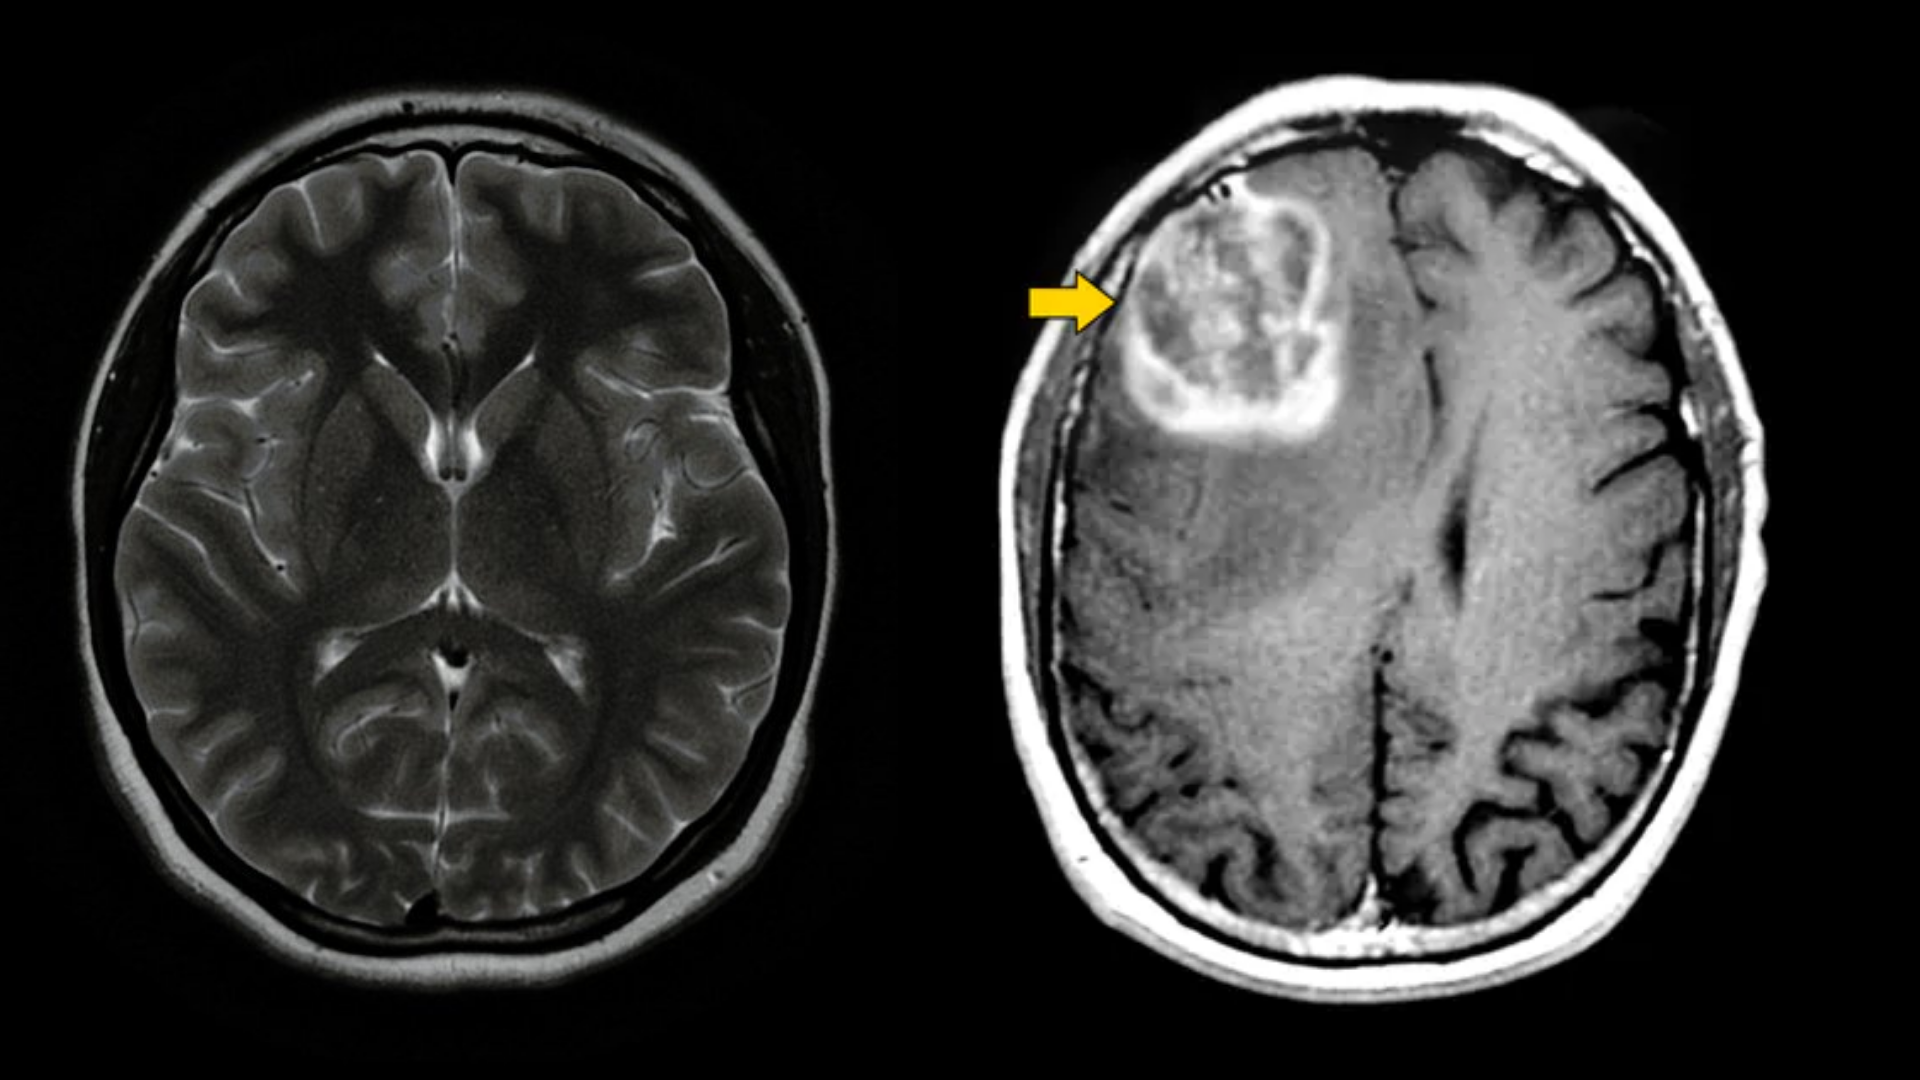
\includegraphics[scale=0.2]{mri.png}
  \caption{MRI Scan of brain without and with tumour} \label{fig:ishan}
\end{figure}
All types of brain tumours evoke some symptoms based on the affected region of the brain. The major symptoms may include headaches, seizures, vision problems, vomiting, mental changes, memory lapses, balance losing etc. Incidence of brain tumours are due to genetics, ionizing radiation mobile phones, extremely low frequency magnetic fields, chemicals, head trauma and injury, immune factors like viruses, allergies, infections, etc. The malignant tumours, also known as cancerous tumours, are of two types - primary tumours which start from the brain, and secondary tumours, which originate somewhere and spread to the brain. The risk factors for brain tumour are exposure to vinyl chloride, neurofibromatosis, ionising radiations and so on. The various diagnostic methods are computed tomography, magnetic resonance imaging, tissue biopsy etc. \par
Better treatments are now available for brain tumours. There is a chance of focal neurological deficits, such as motor deficit, aphasia or visual field defects in the treatment. Side effects can be avoided by measuring tumour size and time to tumour progression (TTP). Estimation of density of affected areas can give a better measurement in therapy. \par
The analysis of brain images is considered imperative because diseases of the brain called brain tumors are fatal and responsible for a large number of deaths in developed countries; for instance, according to the National Brain Tumor Foundation (NBTF), 29,000 people are diagnosed with brain tumor in the United States (US) with brain tumor and 13,000 of those patients die per annum. A number of advanced Magnetic Resonance Imaging (MRI) techniques that include Diffusion Tensor Imaging (DTI), MR Spectroscopy (MRS) and Perfusion MR are used for the analysis of brain tumor through MRI.\par 
Deep learning is a machine learning technique that instructs computers what to do as a human think and do in a scenario. In deep learning, a computer model is able to do classification tasks from images, sound or text. Sometimes human level performance is being exceeded by deep learning techniques. One of the most popular neural networks is an artificial neural network that has a collection of simulated neurons. Each neuron acts as a node and by links each node is connected to other nodes. \par
The aim of this project is to develop a web application that would help in cancer detection from MRI images through the convolution neural network.\\ 

\begin{landscape}
\begin{figure}[H]
  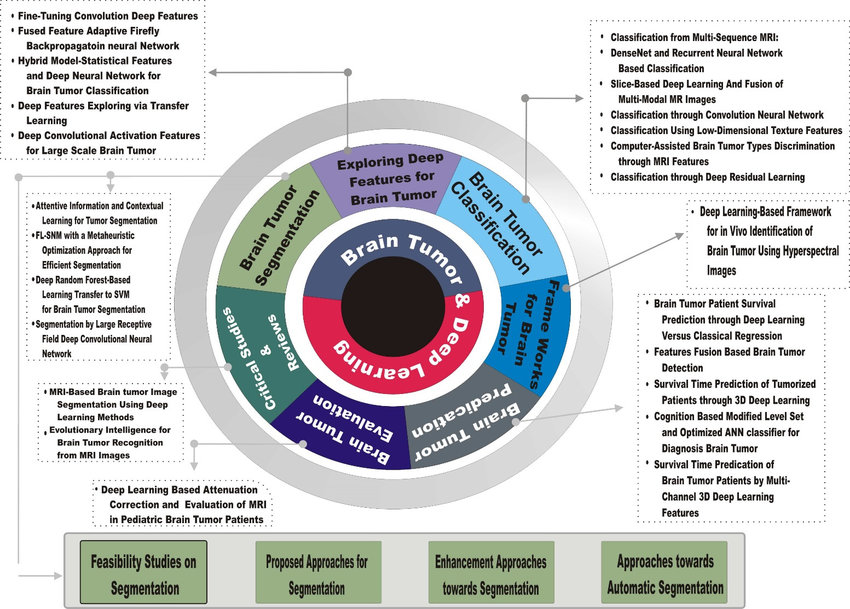
\includegraphics[scale=0.75]{taxonomy_brain.jpg}
  \caption{Literature Taxonomy of brain tumor using deep learning.} \label{fig:ishan}
\end{figure}
\end{landscape}
{\bf \Large Objective and Scope}
\begin{itemize}
    \item To develop a deep learning model for detection of brain tumour from MRI images.
    \item To develop a web application that uses the trained model, which will act as an interface to end users for determining whether the input MRI image has any sort of tumour present in it or not.
    \item To further train the model to classify the type of tumour.
    \item To learn more about Data form analysis and dive into Aritifical intelligence.
\end{itemize}
{\bf \Large Abstract}\par
Brain tumours are a life-threatening problem and hamper the conventional functioning of the shape. For correct diagnosis and efficient treatment planning, it's necessary to detect the brain tumour in the early stages. The tumour within the brain is one of the most dangerous diseases and might be diagnosed easily and reliably with the assistance of detection of the tumour using automated techniques on MRI Images. Positron Emission Tomography, Cerebral Arteriogram, spinal tap, Molecular testing are used for tumour detection. Digital image processing plays an important role in the analysis of medical images. Segmentation of tumours involves the separation of abnormal brain tissues from normal tissues of the brain. Within the past, various researchers have proposed semi and fully automatic methods for the detection and segmentation of tumours . The motivation behind this project is to detect neoplasm and supply better treatment for the suffering. The project uses MRI Scans as the base image for detection purposes.\\
{\bf \Large Project Category}\\
Digital Image Processing, Deep Learning.\\
{\bf \Large Process Description}\\
The web application will use the trained model for detection of brain tumour. This detection model work on pre trained models that are able to analyze the input images provided by the end users. Once the system has input images, it performs pre-processing operations on it. Pre-processing is the name for operations on images at the lowest level of abstraction whose aim is an improvement of the image data that suppress undesired distortions or enhances some image features important for further processing. Some of the steps in the Pre-processing include converting the image to grayscale, detecting the skull and brain part in the MRI image and so on. Once the Pre-processing is done, the system determines whether the input MRI image contains any tumour or not and will intimidate the same to the end users. \\
\begin{figure}[H]
  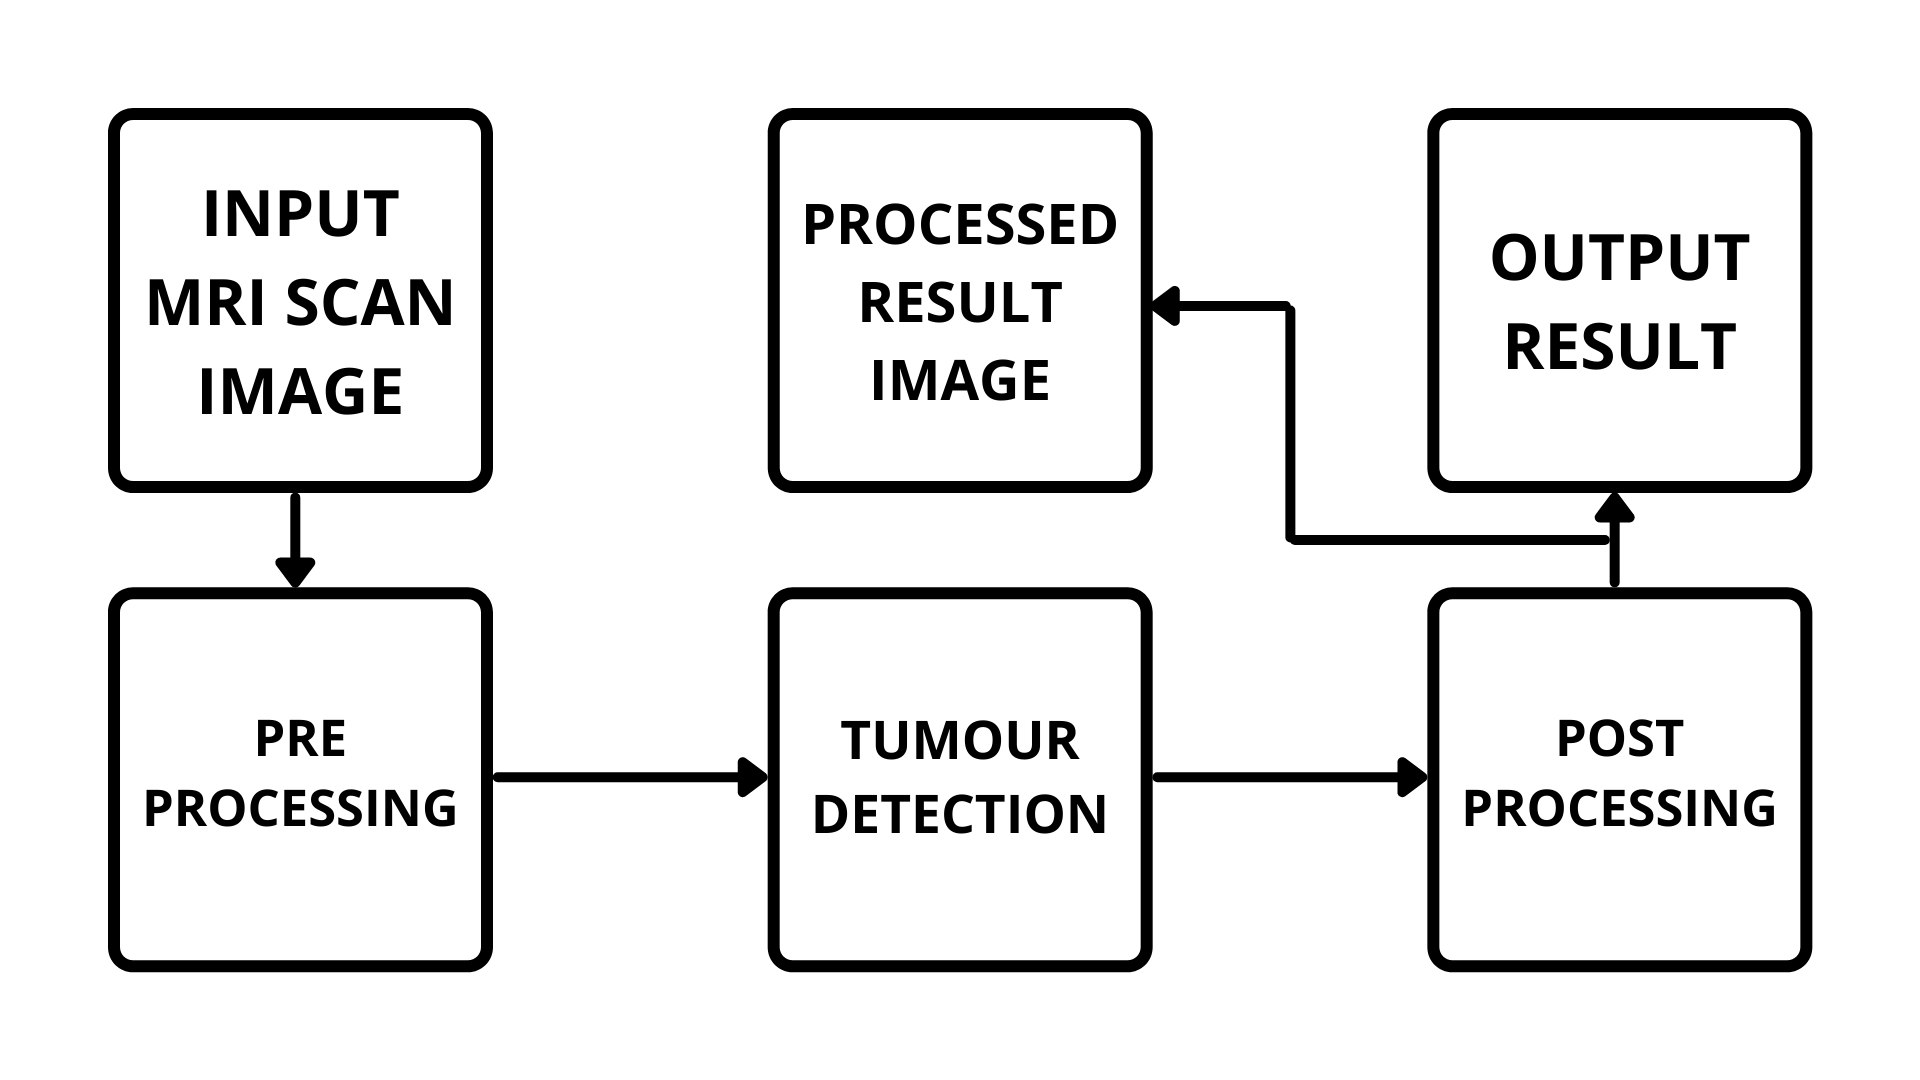
\includegraphics[scale=0.3]{brain_block.png}
  \caption{Proposed Block Diagram} \label{fig:ishan}
\end{figure}
{\bf \Large Requirement of Resources and Limitations}\\
Requirement:
\begin{itemize}
    \item Software Requirement 
        \begin{enumerate}
            \item OS Requirement:
                \begin{itemize}
                    \item Windows 8/10(Can be used both for Training and at User End)
                    \item Linux(Only at User End)
                \end{itemize}
            \item Training of the model:
                \begin{itemize}
                    \item Python ide(Anaconda Jupyter Notebook/Jupyter Lab)
                    \item Dataset for Training
                \end{itemize} 
            \item Web Application
        \end{enumerate}
    \item Hardware Requirement
        \begin{enumerate}
            \item Basic Hardware for Training Purpose:
                \begin{itemize}
                    \item RAM : 8 GB
                    \item ROM : 2 GB
                    \item Processor : i5 Processor
                \end{itemize}
        \end{enumerate}
    \end{itemize}
Limitations: Limited detection due to less datasets being used in training.\\
{\bf \Large Impact analysis}\\
{\textbf{1. Impact of project on society:}}\\
{\textbf{Positive Impact of project on society:}}
\begin{itemize}
    \item Early detection of tumour can reduce the cost required to treat the tumour.
    \item Early detection can overall improve the lifespan of humans.
\end{itemize}\\ 
{\textbf{Negative Impact of project on society:}}
\begin{itemize}
    \item It has a risk of errors and wrong detection due to less training.
    \item It has a risk of not detecting Initial stages of tumour due to small size.
\end{itemize}
{\textbf{2. Impact of project on environment }\\
{\textbf{Positive Impact of project on environment: }}
\begin{itemize}
    \item  Less Bio Medical waste is generated due to early detection and treatment.
\end{itemize}
{\textbf{Negative Impact of project on environment: }}
\begin{itemize}
    \item Bio Medical waste generated during treatment after the detection of tumour is done through this system, if not treated properly can pose environmental risks.
\end{itemize}
{\bf \Large Professional ethical practices to be followed}
\begin{enumerate}
\item Giving credits.
\item Keeping technical guidelines in mind.
\item Following the norms of engineering Practices.
\item Liabality for outcome caused by one's actions or decisions.
\end{enumerate}
{\bf \Large Project Planning (Timeline analysis and Finance management}\\

%{\bf \Large PROJECT PLANNING: (Timing Analysis):}\\
% Please add the following required packages to your document preamble:
% \usepackage{lscape}
% \usepackage{longtable}
% Note: It may be necessary to compile the document several times to get a multi-page table to line up properly
\begin{landscape}
\begin{longtable}[c]{|l|l|l|l|l|l|l|l|l|l|l|l|l|l|}
\caption{PROJECT PLANNING: (Timeline Analysis)}
\label{tab:my-table}\\
\hline
\multicolumn{1}{|c|}{\textbf{Parameters}} &
  \multicolumn{1}{c|}{\textbf{\begin{tabular}[c]{@{}c@{}}Month\\ 1\end{tabular}}} &
  \multicolumn{1}{c|}{\textbf{\begin{tabular}[c]{@{}c@{}}Month\\ 2\end{tabular}}} &
  \multicolumn{1}{c|}{\textbf{\begin{tabular}[c]{@{}c@{}}Month\\ 3\end{tabular}}} &
  \multicolumn{1}{c|}{\textbf{\begin{tabular}[c]{@{}c@{}}Month\\ 4\end{tabular}}} &
  \multicolumn{1}{c|}{\textbf{\begin{tabular}[c]{@{}c@{}}Month\\ 5\end{tabular}}} &
  \multicolumn{1}{c|}{\textbf{\begin{tabular}[c]{@{}c@{}}Month\\ 6\end{tabular}}} &
  \multicolumn{1}{c|}{\textbf{\begin{tabular}[c]{@{}c@{}}Month\\ 7\end{tabular}}} &
  \multicolumn{1}{c|}{\textbf{\begin{tabular}[c]{@{}c@{}}Month\\ 8\end{tabular}}} &
  \multicolumn{1}{c|}{\textbf{\begin{tabular}[c]{@{}c@{}}Month\\ 9\end{tabular}}} &
  \multicolumn{1}{c|}{\textbf{\begin{tabular}[c]{@{}c@{}}Month\\ 10\end{tabular}}} &
  \multicolumn{1}{c|}{\textbf{\begin{tabular}[c]{@{}c@{}}Month\\  11\end{tabular}}} &
  \multicolumn{1}{c|}{\textbf{\begin{tabular}[c]{@{}c@{}}Month\\  12\end{tabular}}} \\ \hline
\endhead
%
\textbf{\begin{tabular}[c]{@{}l@{}}Formation of \\ group\end{tabular}}                 &\cellcolor{blue!25}Y &  &  &  &  &  &  &  &  &  &  &  \\ \hline
\textbf{\begin{tabular}[c]{@{}l@{}}Identification of\\ problem statement\end{tabular}} &  & \cellcolor{blue!25}Y &  &  &  &  &  &  &  &  &  &    \\ \hline
\textbf{\begin{tabular}[c]{@{}l@{}}Literature \\ survey\end{tabular}}                  &  & \cellcolor{blue!25}Y & \cellcolor{blue!25}Y &  &  &  &  &  &  &  &  &   \\ \hline
\textbf{\begin{tabular}[c]{@{}l@{}}Objectives and \\ outcomes\end{tabular}}            &  &  & \cellcolor{blue!25}Y &  &  &  &  &  &  &  &  &    \\ \hline
\textbf{\begin{tabular}[c]{@{}l@{}}Proposed system \\ (methodology)\end{tabular}}      &  &  &  &\cellcolor{blue!25}Y  &  &  &  &  &  &  &  &    \\ \hline
\textbf{\begin{tabular}[c]{@{}l@{}}Simulation/ \\ Testing)\end{tabular}}   &  &  &  &  &\cellcolor{blue!25}Y  & \cellcolor{blue!25}Y & \cellcolor{blue!25}Y &  &  &  &  &    \\ \hline
\textbf{\begin{tabular}[c]{@{}l@{}}Developing final \\ product\end{tabular}}    &  &  &  &  &  &  &  & \cellcolor{blue!25}Y & \cellcolor{blue!25}Y &  &  &   \\ \hline
\textbf{\begin{tabular}[c]{@{}l@{}}Testing and \\ verification\end{tabular}}           &  &  &  &  &  &  &  &  &  & \cellcolor{blue!25}Y &  &    \\ \hline
\textbf{\begin{tabular}[c]{@{}l@{}}Report \\ writing\end{tabular}}                     &  &  &  &  &  &  &  &  &  &  & \cellcolor{blue!25}Y & \cellcolor{blue!25}Y   \\ \hline
\textbf{\begin{tabular}[c]{@{}l@{}}Final presentation/\\  demo\end{tabular}}           &  &  &  &  &  &  &  &  &  &  &  & \cellcolor{blue!25}Y \\ \hline
\multicolumn{14}{|l|}{(color the cells selected for the task/parameter to be perform} \\ \hline
\end{longtable}
\end{landscape}
{\bf \Large Future scope and further enhancement}\\
\begin{enumerate}
\item The entire Web Application can be further developed to understand more types of human body scans such as X-ray, CT - Scans etc. So as to become a full fledged health assessment portal.
\item Such web application could be installed at hospitals which will then connect patients and the hospital staff virtually.
\item The system in it's base form can be trained further to detect the tumour even more efficiently.
\item The system can be upgraded to detect more types of tumours such as ovarian, breast, skin, lung tumours etc.
\end{enumerate}
{\bf \Large Expected Outcome}\\
A web application that uses trained models to detect whether a patients or test MRI Scan Image has any signs of tumour. If there is any tumour detected, the system is to alert the user for the same.\\ 
